\section{System description}
\label{sec:sys}

This section will present a detailed description of our \ac{LTR} system. 
Our system was designed to work by using 3D lidar scans as a primary mean of localization, also using \ac{IMU} and wheel odometry as input. 
The main components of the framework are shown in~\autoref{fig:ltr_flow}.
As the \ac{ICP} algorithm is the foundation of this algorithm, our implementation of the \ac{ICP} algorithm is detailed first. 
Next, the teach phase is described, explaining how the reference trajectory and map are logged.
Subsequently, the repeat phase is described, when the robot localizes within the map a simple controller allows computing commands that allow to repeat the reference trajectory.
Finally, the hardware used to deploy the \ac{LTR} system, including the \ac{UGV}, sensing and computing hardware is described.

\begin{figure} [htpb]
	\centering
	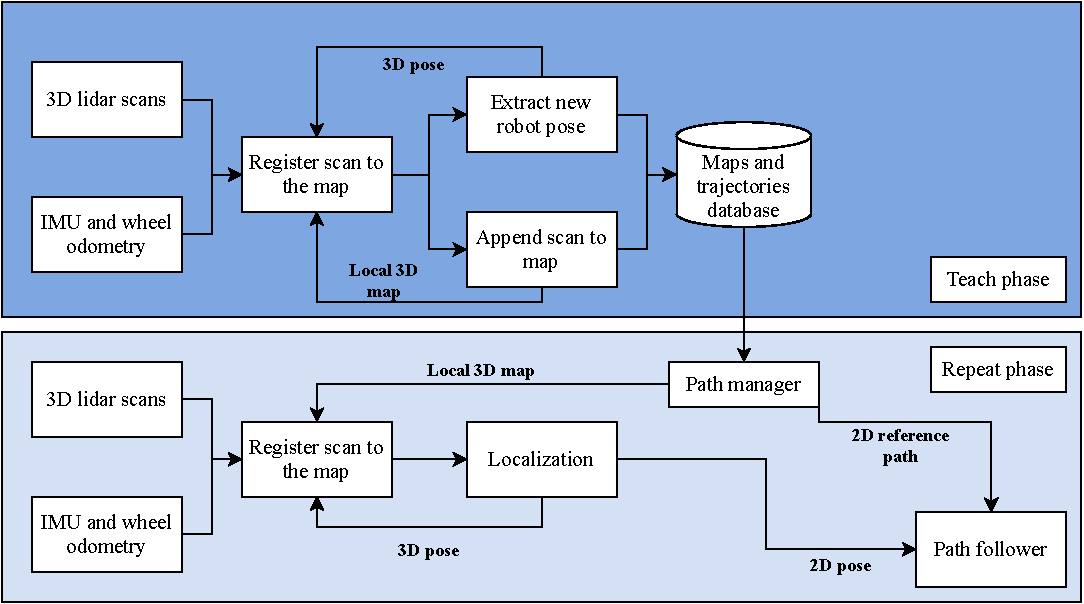
\includegraphics[height=3.2in]{figs/LTR_flowchart.pdf}
	\caption{Flowchart for LTR}
	\label{fig:ltr_flow}
\end{figure}

Various coordinate frames need to be defined for the \ac{LTR} framework to work, all of which are illustrated in~\autoref{fig:ltr_frames}.
First, a map frame $\mapf$ is defined representing the world in which the robot is navigating.
Second, an odom frame $\odomf$ is defined in order to localize the robot at a higher frequency. %JL: odom -> odometry?
The rigid transform between from the odom frame $\odomf$ to the map frame %unfinished sentence ;) 
A robot frame $\robotf$ is defined at the base of the robot chassis. 
The rigid transform from the odom frame to the map frame \transform{\odomf}{\mapf} is updated every time a new localization is computed by the \ac{ICP} algorithm.
Thirdly, a robot frame $\robotf$ is defined with its origin at the base of the robot chassis and the $x$-axis parallel to the longitudinal direction and the $y$-axis parallel to the lateral direction of the vehicle.
The rigid transform \transform{\robotf}{\odomf} is updated at the rate of the \ac{IMU} and wheel odometry and used as a prior for the \ac{ICP} algorithm.
Fourthly, a lidar frame $\lidarf$ is defined at the origin of the lidar sensor. 
The rigid transform from the lidar frame to the robot frame \transform{\lidarf}{\robotf} is assumed to be constant and found through system calibration.
Reading point clouds $\readpc$ are originally observed in the lidar frame $\lidarf$ but are then expressed in the map frame $\mapf$ by chaining rigid transformations from the lidar frame to the map frame \transform{\lidarf}{\mapf}.

%% TODO : Replace with our version of the figure
\begin{figure} [htpb]
	\centering
	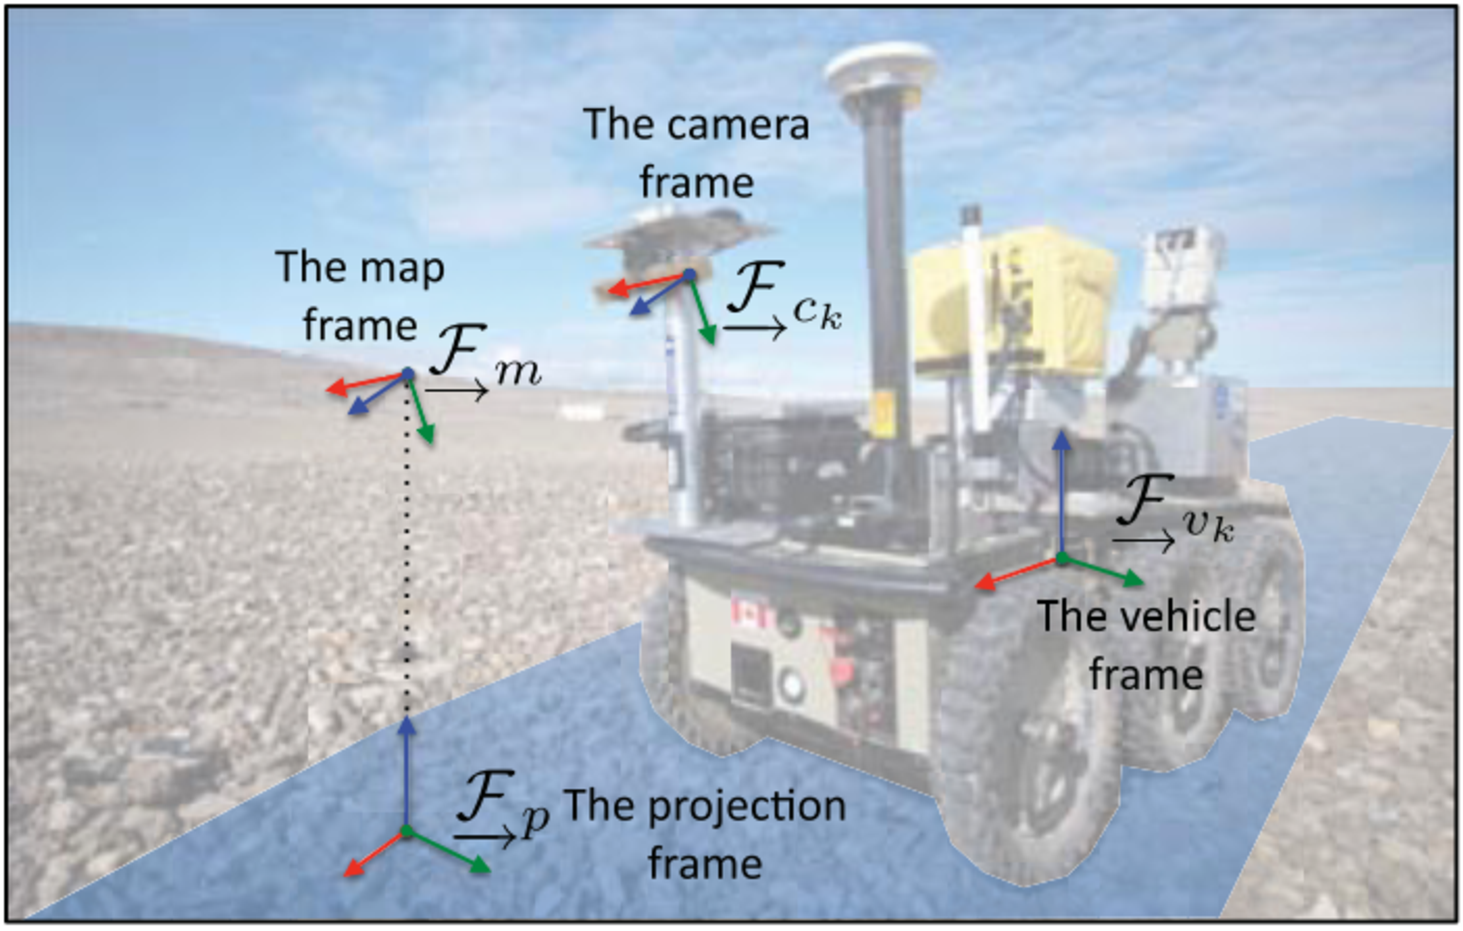
\includegraphics[height=2.0in]{figs/warthog_frames.pdf}
	\caption{Coordinate frames used for \ac{LTR}}
	\label{fig:ltr_frames}
\end{figure}

\subsection{Iterative closest point}
\label{ICP}

Incoming lidar scans, or reading point clouds $\readpc$ registered to a reference map, or reference point cloud $\refpc$ using the \ac{ICP} algorithm in order to localize the robot and build a map of the environment during the teach phase.

%% TODO : Re-do this figure to suit our needs for the paper
\begin{figure} [htpb]
	\centering
	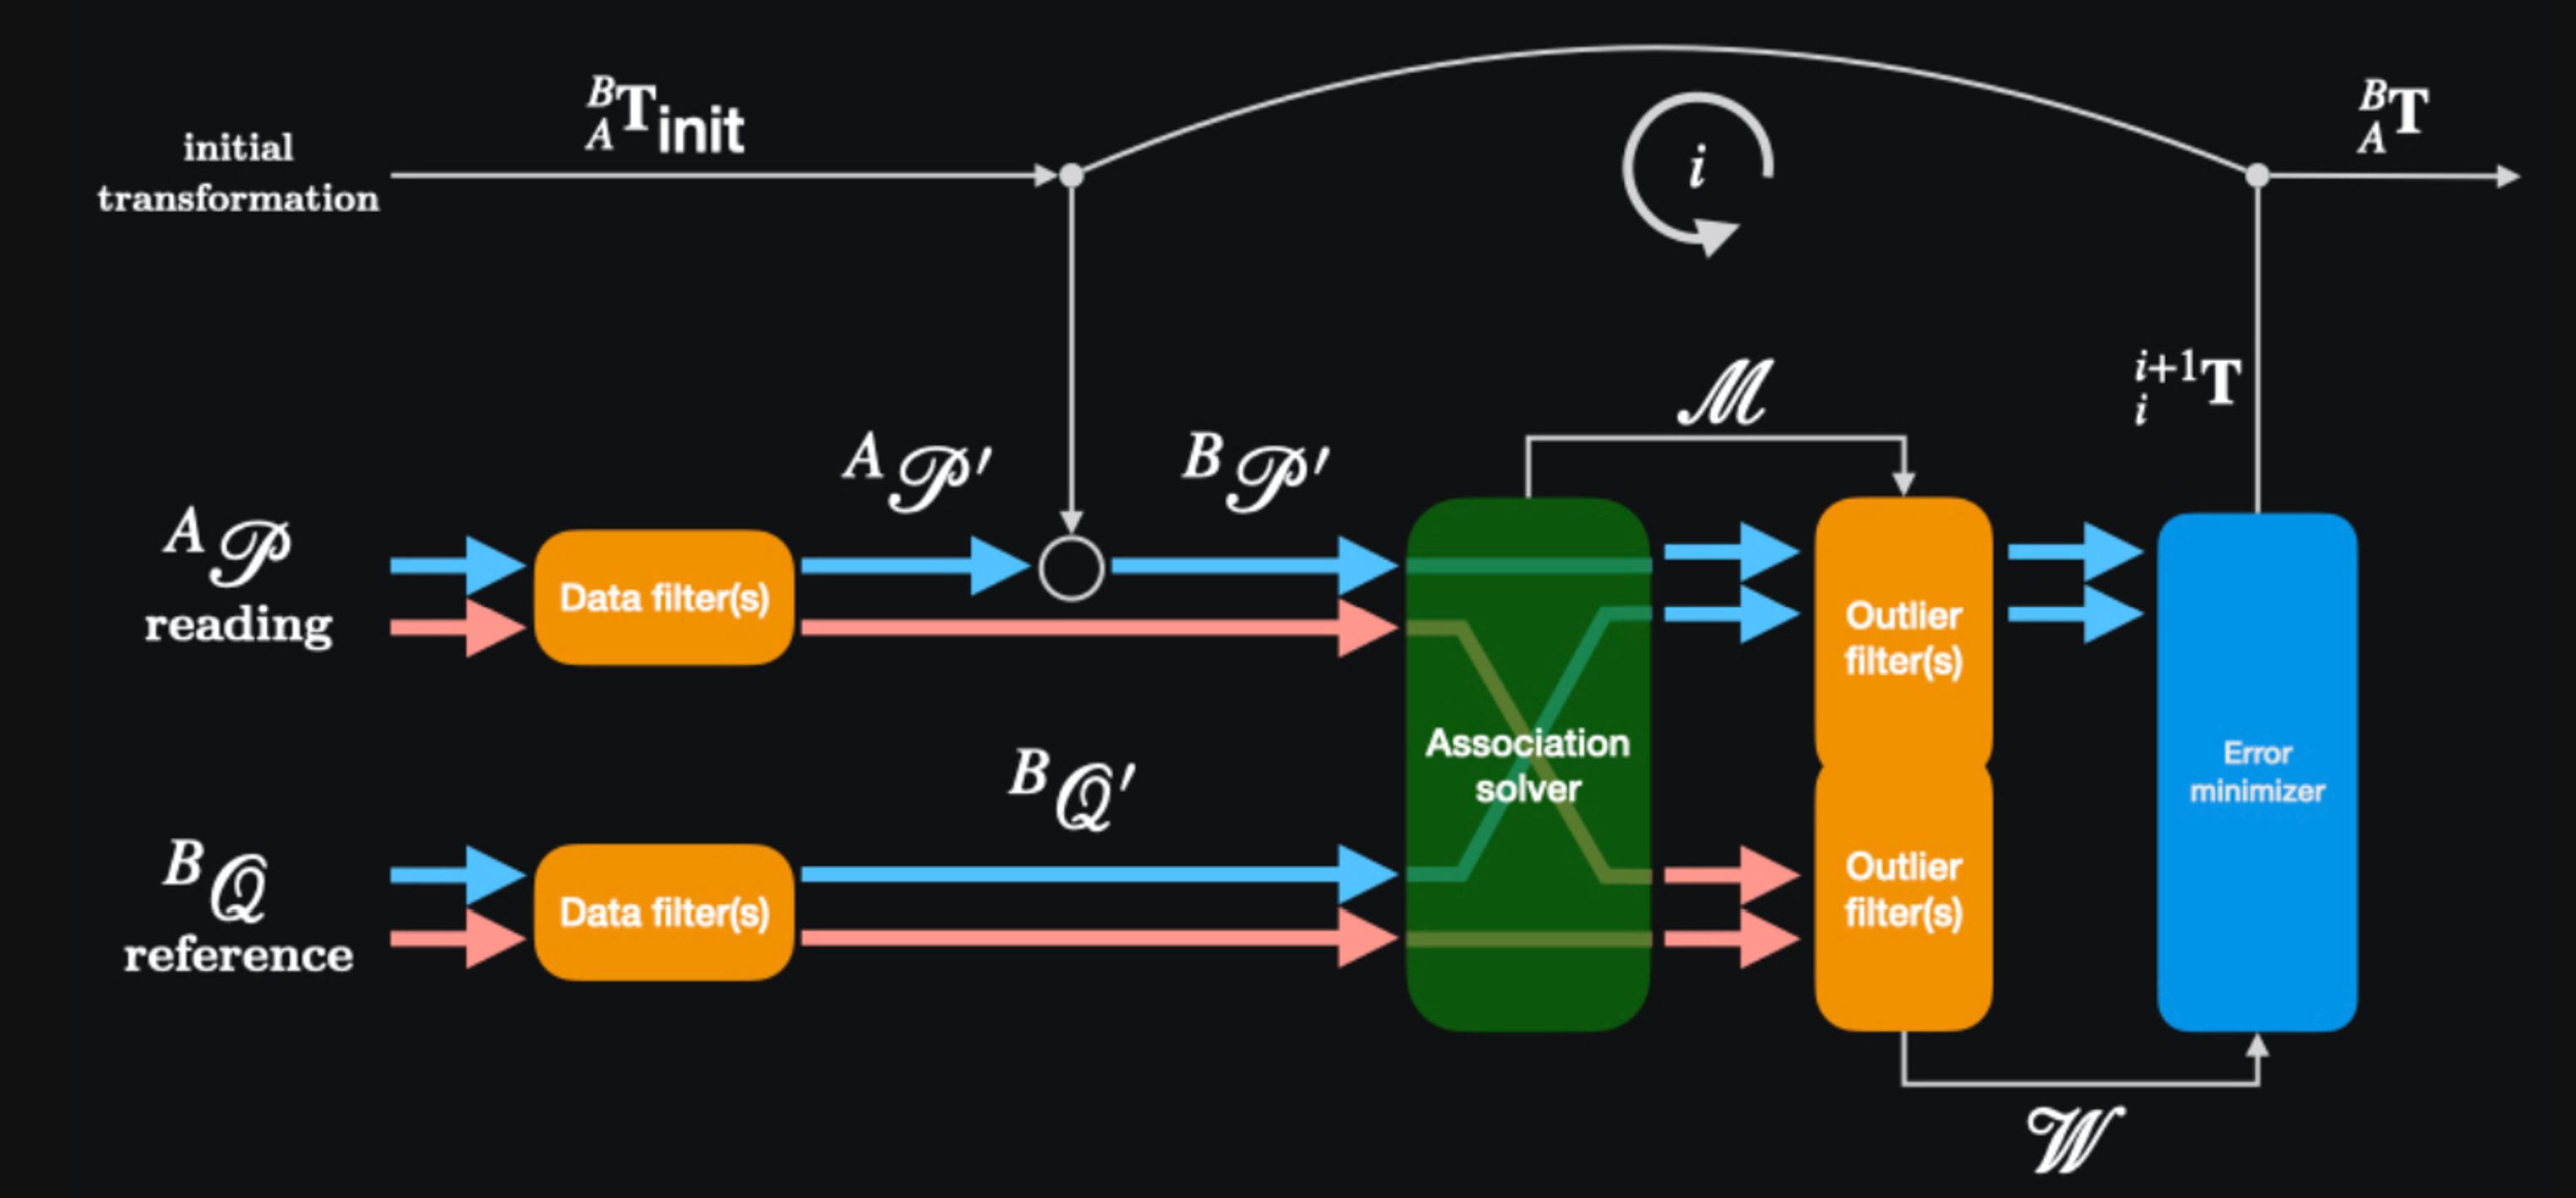
\includegraphics[height=2.0in]{figs/icp_pipeline.pdf}
	\caption{ICP pipeline}
	\label{fig:icp_pipeline}
\end{figure}

\subsubsection{Tiled mapping for large scale}
\label{sec:tiled_map}
\lightlipsum[1]

\begin{figure} [htpb]
	\centering
	\includegraphics[height=2.0in]{example-image}
	\caption{Figure explaining Simon-Pierre's tiled mapping framework}
	\label{fig:tiled_map}
\end{figure}


\begin{table}[htpb]
	\caption{\ac{ICP} parameters} \label{tab:LTR-runs}
	\begin{center}
		\begin{tabular}{|c|c|c|c|c|c|}
			\hline
			% after \\: \hline or \cline{col1-col2} \cline{col3-col4} ...
			& $k_{g}$ & $k_{o}$ & $c_{3}$ & $c_{4}$ & $c_{5}$ \\
			\hline\hline
			Careful/Sparse & 0.334 & 0.597 & 1.101 & 9.621 & 8.170 \\ \hline
			Careful/Dense & 3.124 & 3.195 & 1.094 & 5.899 & 7.318 \\ \hline
			Aggressive/Sparse & 0.840 & 9.153 & 2.853 & 8.274 & 0.187 \\ \hline
			Aggressive/Dense & 4.838 & 2.841 & 0.670 & 7.952 & 0.386 \\ \hline
			Hand-Tuned & 0.767 & 0.060 & 0.340 & 2.000 & 0.250 \\
			\hline
		\end{tabular}
	\end{center}
\end{table}

\subsection{Teach phase}
\label{sec:teach_phase}

During the teach phase
\lightlipsum[1]

\begin{figure} [htpb]
	\centering
	\includegraphics[height=2.0in]{example-image}
	\caption{Teach phase pipeline}
	\label{fig:teach_pipeline}
\end{figure}

\subsection{Repeat phase}
\label{sec:repeat_phase}

\lightlipsum[1]

\begin{figure} [htpb]
	\centering
	\includegraphics[height=2.0in]{example-image}
	\caption{Repeat phase pipeline}
	\label{fig:repeat_pipeline}
\end{figure}

\subsubsection{Repeat localization}
\label{sec:rep_loc}

\lightlipsum[1]

\subsubsection{Path following}
\label{sec:orthexp}

%% Review Frenet-Serret frame formulation from Huskic 2019

Once the robot is localized within the environment and the reference trajectory is defined, this information is used as input to a simple path following controller in order to complete the repeat pipeline.
The output of the path-following algorithm is the commanded longitudinal and angular velocities, defined in the vector $\bm u = [v_x, \omega]$.
For our implementation, we selected a simple \ac{ORTHEXP} controller. 
Originally proposed by~\citet{Mojaev2004} for differential-drive mobile robots, this controller allows path tracking with a feedback loop on robot localization.
This controller was later adapted for omnidirectional mobile robots by~\citet{Li2007} and for dribbling control for soccer robots.
More recently,~\citet{Huskic2017} improved the algorithm's path following performance through heuristic linear velocity control.
To implement this controller, we used the open-source \ac{GeRoNa} library, created by~\citet{Huskic2019}.

Knowing the robot's 2D pose $\bm x_{\text{2D}}$ and reference trajectory $\bm x_{\text{ref}}$, it is possible to compute the orthogonal projection $\bm P$ of the robot on the reference path. %JL: I think it's better to always use \text{} or \texttt, mathtt or other while writing several letters in math, otherwise it's simply considered as one variable per letter. changed 2D by \text{2D} and ref by \text{ref}
A path reference frame $\pathf$ is defined within the map frame with its origin corresponding to the point $\bm P$.
For the path reference frame, abscissa $\bm x_t$ and ordinate $\bm x_n$ are unit tangent and unit normal vectors respectively. 
The orthogonal distance from the origin of the robot frame $\robotf$ and the path frame $\pathf$ along the $\bm x_n$ axis is denoted with $x_n$ and the tangential distance with $x_t$.
The tangential angle of the path frame $\pathf$ with respect to the map frame $\mapf$ is defined as $\theta_t$.
The angle of robot frame $\robotf$'s $\bm x$ axis with respect to the map frame $\mapf$ is defined $\theta_r$. %JL robot frame R's -> hard to read
If we denote $x_{n_o}$ as the distance between the origin of the robot frame $\robotf$ and the origin of the path frame $\pathf$, it is possible to define the following exponential law as
\begin{equation}
\label{eq:exp_law}
	x_n = x_{n_o} e^{-k x_t},
\end{equation}
where $k$ is a positive constant that allows to regulate the convergence speed of the robot to the path.
Next, the exponential function's tangent angle with the map frame $\phi_e$ can be computed as follows:
\begin{equation}
\label{eq:exp_angle}
\phi_e = \arctan(-k x_n).
\end{equation}

The angular velocity command can then be computed as %JL: remove some "as follows" before the equation and added punctuation 
\begin{equation}
\label{eq:exp_PD}
	\omega = K_h (\phi_e + \theta_e),
\end{equation}
where $\theta_e$ is the error between the robot angle $\theta_r$ and the path frame angle $\theta_t$.
The $K_h$ parameter is a gain on commanded angular velocity that was added after we empirically observed that the robot stabilizes at an angular velocity significantly lower than the commanded angular velocity, based on \ac{IMU} measurements.
A summary of the geometrical representation of the variables affecting the angular velocity command is shown in~\autoref{fig:diff_orthexp}.

% TODO : Replace with our own version of this figure
\begin{figure} [htpb]
	\centering
	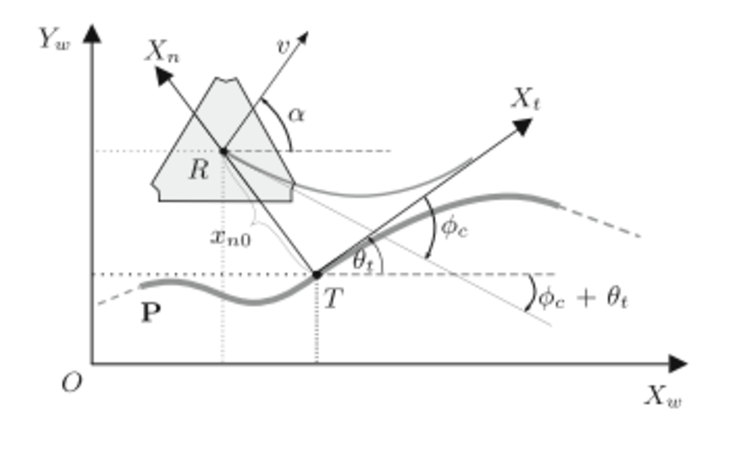
\includegraphics[height=2.5in]{figs/orthexp.pdf}
	\caption{Figure explaining Differential orthogonal-exponential controller}
	\label{fig:diff_orthexp}
\end{figure}

In the \ac{GeRoNa} library, commanded longitudinal velocity $v_x$ can be computed based on multiple factors such as upcoming path curvature, current vehicle angular velocity, proximity of obstacles and distance from the end goal.
Due to \ac{ICP} localization noise in the teach phase, the upcoming path curvature would sometimes peak causing the robot to stop on the spot, we therefore removed this factor.
Current vehicle angular velocity has also been removed from the equation to simplify controller parameter tuning.
In our system, no obstacle detection feature is included, meaning that the proximity of obstacles cannot be used as a factor to compute linear velocity.
It is only the distance from the end goal that was used in order to prevent the robot from finishing its course abruptly.
Thus, the commanded linear velocity $v_x$ is computed as
\begin{equation}
\label{eq:exp_lin_vel}
v_x = v_n \exp\left(-\left(\frac{K_g}{d_g}\right)\right),
\end{equation}
where $v_n$ is the target vehicle velocity and $d_g$ is the distance between the robot's pose and the last pose of the final reference trajectory pose. 
At each time step, a new exponential function and command $\bm u$ are computed using the control laws shown in~\autoref{eq:exp_PD} and~\autoref{eq:exp_lin_vel}, using the robot's 2D pose $x_{\text{2D}}$ and reference trajectory $\bm x_{\text{ref}}$ as input.
The parameters for the \ac{ORTHEXP} controller were tuned empirically by having the robot repeating arbitrary short trajectories and minimizing error, these parameters are detailed in~\autoref{tab:orthexp_params}.


\begin{table}[htpb]
	\caption{\ac{ORTHEXP} controller parameters} \label{tab:orthexp_params}
	\begin{center}
		\begin{tabular}{c c | c c | c c}
			% after \\: \hline or \cline{col1-col2} \cline{col3-col4} ...
			General & & Angular velocity & & Linear velocity \\
			\hline
			Waypoint tolerance & \SI{1.0}{m} & $k$ & 0.4 & $K_g$ & 0.5 \\
			Goal tolerance & \SI{0.15}{m} & $K_g$ & 0.5 & $v_n$ & \SI{1.5}{m/s} \\
			 & & $K_h$ & 3.0 & $v_{min}$ & \SI{0.5}{m/s} \\
			 & & Max angular velocity & \SI{1.0}{rad/s} & $v_{max}$ & \SI{1.5}{m/s} \\
			\hline
		\end{tabular}
	\end{center}
\end{table}

\subsection{Hardware description}
\label{sec:hardware}

Our system was deployed on a Clearpath Robotics Warthog \ac{UGV}. 
The Warthog is a \ac{SSMR} using two drive units located on each side of its chassis. 
For \acp{SSMR}, steering is done by sending rotating the wheels on each side of the vehicle at different velocities to creating a skidding effect, effectively turning the vehicle.
The Warthog can be equipped with wheels or tracks, for this work, we selected the latter in order to maximize mobility. 
The Warthog is also equipped with a differential suspension, maximizing track or wheel traction when navigating steep terrain.
The warthog is also equipped with a standard sensor suite for autonomous navigation. 
In order to enable the \ac{LTR} framework, a Robosense RS-32 3D lidar is mounted in front of the robot, for this work, it is the only lidar used for localization.
3 Hall effect sensors are added to each motor to provide wheel odometry for the robot. 
Finally, an XSens MTi-10 \ac{IMU} provides angular velocity, body linear acceleration and gravitational acceleration measurements. 
Additional sensors used for recording in this work include a Dalsa C1920 camera and two Emlid Reach-RS+ \ac{GPS} receivers.
Two Robosense RS-16 lidars were added to the rear of the platform to collect measurements on tree canopy but no data was recorded through those sensors. 
All technical specifications for the platform are given in~\autoref{tab:warthog_specs}.

\begin{table}[htpb]
	\caption{Warthog specifications} \label{tab:warthog_specs}
	\begin{center}
		\begin{tabular}{c c | c c}
			\textbf{Physical} &  & \textbf{Power} & \\
			% after \\: \hline or \cline{col1-col2} \cline{col3-col4} ...
			Mass & \SI{590}{kg} & Chemistry & AGM sealed lead acid \\ 
			Footprint & 2.13 x 1.52 m & Voltage & \SI{48}{V} \\ 
			Top speed & \SI{18}{km/h} & Capacity & \SI{105}{Ah} \\ 
			Steering geometry & Skid-steering  & Drive & Sevcon Gen4 \\
			Locomotion & CAMSO ATV T4S Tracks \\
			Suspension & Geometric Passive Articulation \\
			\hline
			\textbf{Sensors} & & \textbf{Computing} \\
			\ac{LTR} & & Computer & Acrosser AIV-Q170V1FL  \\
			Front lidar & Robosense RS-32 (\SI{10}{Hz}) & CPU & i7-6700 TE \\
			\ac{IMU} & XSens MTi-10 (\SI{100}{Hz}) \\ 
			Wheel encoders & 3 x hall effect sensors (\SI{4}{Hz}) \\
			Recording & &   \\
			Camera & Dalsa C1920 (\SI{8}{Hz})  \\
			\ac{GPS} & Emlid Reach-RS+ (\SI{5}{Hz}) \\
		\end{tabular}
	\end{center}
\end{table}

\begin{SCfigure}
	\centering
	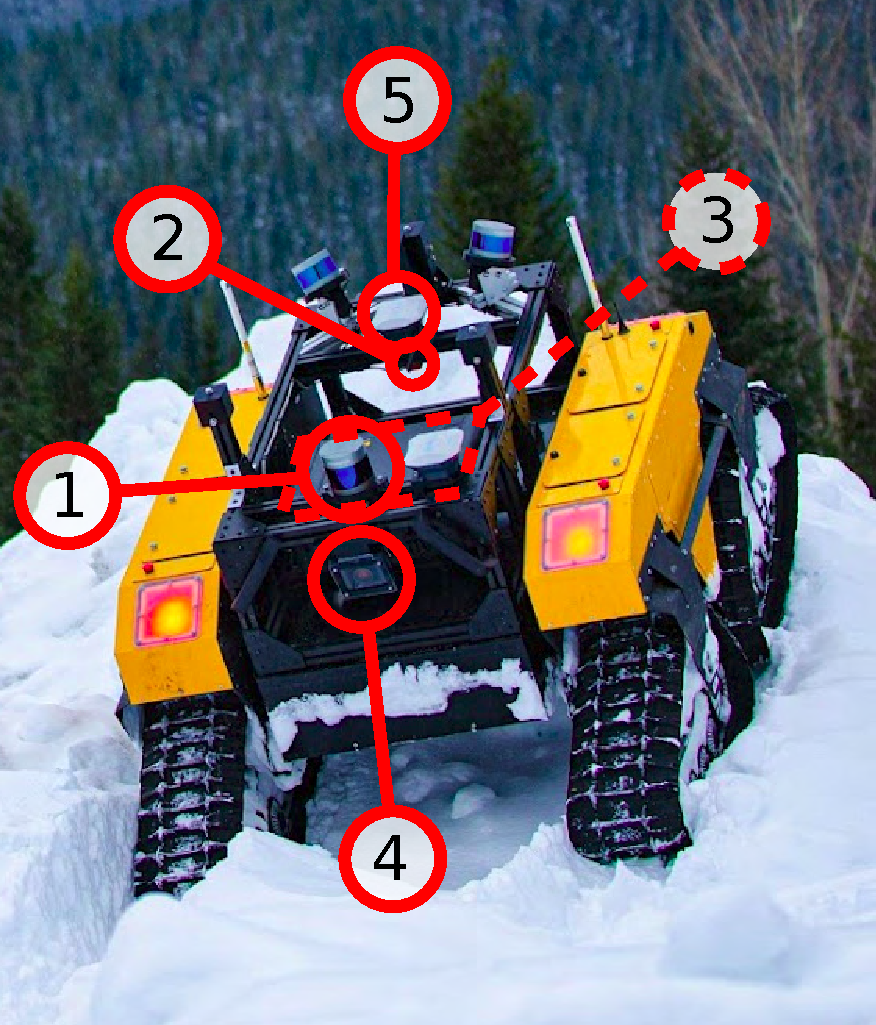
\includegraphics[height=2.5in]{figs/warthog_hardware.pdf}
	\caption{The experimental setup for \ac{LTR} on our Clearpath Robotics Warthog \ac{UGV}: (1) Robosense RS-32 lidar, (2) XSens MTi-10 \ac{IMU}, (3) Acrosser AIV-Q170V1FL computer, (4) Dalsa C1920 color camera, (5) 2 Emlid Reach-RS+ \ac{GPS} antennas.}
	\label{fig:warthog}
\end{SCfigure}
%% To do : Edit Figure to add pointers for all sensors
